\documentclass[11pt,a4paper]{memoir}

\usepackage[utf8]{inputenc}
\usepackage[T1]{fontenc}
\usepackage{geometry}
\geometry{margin=2.5cm}
\usepackage{hyperref}
\usepackage{listings}
\usepackage{xcolor}
\usepackage{graphicx}
\usepackage{amsmath, amssymb}
\usepackage{booktabs}
\usepackage{subcaption}

\hypersetup{
    colorlinks=true,
    linkcolor=blue,
    citecolor=blue,
    urlcolor=blue
}

\title{\textbf{Distributed Systems Project: \\ Permissioned Blockchain Inventory System}}
\author{\textbf{Cancian Matteo} \quad \and \quad \textbf{Del Pio Luogo Marco}}
\date{Version 0.3 --- \today}

\begin{document}

\maketitle

\begin{abstract}
Managing inventory across multi-site enterprise environments presents critical challenges regarding data integrity, traceability, and accountability. 
Traditional centralized hierarchical systems introduce single points of failure and rely on trusted administrators who can unilaterally modify audit logs. 
This project proposes a fault-tolerant, permissioned blockchain-based distributed system for enterprise asset tracking. The system guarantees immutable, append-only logging of inbound and outbound inventory transactions while supporting human error remediation through cryptographic compensating operations. Operating over a network with fair-loss links under a synchronous model, the platform leverages Proof of Authority (PoA) and Byzantine Fault Tolerance (BFT) consensus to achieve deterministic block finality, high throughput, and resilience against adversarial node behavior.
\end{abstract}

\clearpage
\tableofcontents
\clearpage

% ==============================================================================
% CHAPTER 1: INTRODUCTION
% ==============================================================================
\chapter{Introduction}\label{ch:intro}

\section{Application Overview and Problem Statement}
In modern enterprise environments operating across geographically distributed sites (like national or continental logistics hubs), managing inventory with high reliability is a primary operational requirement. 
Organizations must track every item movement seamlessly, covering two fundamental workflows:
\begin{itemize}
    \item \textbf{Inbound Operations:} Recording newly arrived goods or asset creations into the global inventory system.
    \item \textbf{Outbound Operations:} Documenting the dispatch, sale, or permanent removal of assets from the inventory.
\end{itemize}

Centralized inventory databases suffer from fundamental vulnerabilities and limitations. 
A compromised system administrator or external attacker can alter historical logs, modify asset quantities retroactively, or erase operational records without detection. 
Furthermore, centralized infrastructures represent Single Points of Failure (SPF) vulnerable to hardware faults, network partitioning, and physical disasters.

Conversely, human operators and automated IoT scanners inevitably commit operational errors (misscanning barcodes, miskeying quantities, or logging duplicate items). 
In an immutable ledger, simply deleting or modifying past entries is forbidden by design. 
So, a robust distributed inventory system must provide a mechanism for \textit{error remediation} through explicit, auditable compensating transactions without compromising historical integrity.

\section{Proposed Solution: Permissioned Blockchain Architecture}
To address these challenges, we design a distributed inventory management platform backed by a \textbf{Permissioned (Consortium) Blockchain}. Unlike public permissionless blockchains (e.g., Bitcoin or Ethereum), where unknown participants compete via energy-intensive Proof of Work (PoW), a permissioned blockchain restricts ledger validation to pre-authorized enterprise nodes.

The system relies on two primary node types:
\begin{enumerate}
    \item \textbf{Validator/Blockchain Nodes:} Enterprise servers deployed at key regional headquarters or trusted data centers. They maintain the full replicated ledger, run distributed consensus protocols, validate incoming transaction payloads, and assemble transactions into sequential blocks.
    \item \textbf{Client/Operator Nodes:} User-facing client terminals (web frontends or handheld devices) utilized by warehouse staff. Client nodes do not participate in block generation; instead, they sign transactions locally and submit them to validator nodes via API endpoints.
\end{enumerate}

By storing item movements as cryptographically signed transaction logs linked through cryptographic hashes ($H(B_n) = \text{Hash}(B_{n-1} \parallel T_n \parallel \text{nonce})$), the system ensures strict sequential ordering, immutability, and full accountability. 

In this project, we omitted the implementation of \textbf{strong authentication methods} for the 'operator'. We therefore assume that transactions are authentically signed by the operators, making it impossible for a Byzantine node to alter them. 

\section{Trade-off Analysis of Blockchain Technology}
Applying blockchain technology to enterprise asset management introduces distinct advantages alongside technical trade-offs, summarized below.

\subsection{Advantages}
\begin{itemize}
    \item \textbf{Immutability and Anti-Tampering:} Once a block is committed through consensus, retroactively modifying a transaction requires re-executing consensus across the majority of validator nodes, making fraud virtually impossible.
    \item \textbf{Complete Historical Traceability:} The chain provides an unbroken audit log for every asset from initial registration (inbound) to final disposal (outbound), eliminating operational disputes between warehouse sites.
    \item \textbf{High Infrastructure Resilience:} Replicating the state across independent regional validator nodes guarantees high availability; the failure or destruction of a single site does not cause data loss or system downtime.
\end{itemize}

\subsection{Disadvantages and Mitigations}
\begin{itemize}
    \item \textbf{Error Remediation Complexity:} Because records cannot be erased, mistake correction requires introducing new explicit compensating transactions (e.g., explicit reversals) linked to the original erroneous transaction ID.
    \item \textbf{Latency vs Throughput:} Distributed consensus introduces message overhead compared to traditional relational databases. Using Proof of Authority (PoA) minimizes this performance cost.
\end{itemize}

\section{Consensus Mechanism: Proof of Authority (PoA)}
Because all validator nodes represent known corporate entities, consensus is achieved via \textbf{Proof of Authority (PoA)} and leader-based Byzantine Fault Tolerance (BFT) algorithms (e.g., PBFT). 

In PoA, round-robin or stake-weighted validator rotations designate a block proposer for each time interval. The proposer aggregates pending transactions, signs the proposed block, and broadcasts it to peer validators. Peer nodes verify the proposer's digital signature and the validity of all contained transactions before appending the block to their local copy of the ledger.

\section{Testing Plan and Project Schedule}
\subsection{Testing Strategy}
\begin{itemize}
    \item \textbf{Unit Testing:} Verification of modules and functions independently through specific test suites. 
    \item \textbf{Integration Testing:} Testing client-to-validator communication, transaction propagation, and state machine transitions.
    \item \textbf{System \& Fault Tolerance Testing:} Simulating node crashes, network packet loss, message reordering, and malicious/Byzantine transaction proposals.
\end{itemize}

\subsection{Project Schedule}
The project design and implementation follow a four-stage timeline:
\begin{enumerate}
    \item \textbf{Phase 1 (Requirements \& Architecture):} Defining system specifications, network models, and UML sequence diagrams.
    \item \textbf{Phase 2 (Core Development):} Implementing the permissioned blockchain node, networking functionlities, and basic consensus mechanism.
    \item \textbf{Phase 3 (Client Layer):} Developing client APIs, operator UI, and compensating transaction handling.
    \item \textbf{Phase 4 (Validation \& Evaluation):} Conducting benchmark simulations, network failure injection, and report finalization.
\end{enumerate}

% ==============================================================================
% CHAPTER 2: ANALYSIS
% ==============================================================================
\chapter{Analysis}\label{ch:analysis}

In this chapter, we outline the functional and non-functional requirements for the proposed blockchain inventory system.

\section{Functional Requirements}

\begin{description}
    \item[\textbf{FR-1: Inbound Items Registration}]\hfill
    \begin{itemize}
        \item \textbf{Description:} Allows an authorized operator to register new assets into the global inventory.
        \item \textbf{Input:} Asset details (ID, description, batch number, quantity, location), operator signature.
        \item \textbf{Output:} Transaction hash and confirmation of block inclusion.
        \item \textbf{Effect:} Increases global asset count; creates initial cryptographic provenance record on the ledger.
    \end{itemize}

    \item[\textbf{FR-2: Outbound Items Tracking}]\hfill
    \begin{itemize}
        \item \textbf{Description:} Registers the dispatch or removal of existing assets from stock.
        \item \textbf{Input:} Asset ID, quantity removed, destination details, operator signature.
        \item \textbf{Output:} Transaction receipt or error notification (if insufficient stock exists).
        \item \textbf{Effect:} Appends outbound movement record to the chain.
    \end{itemize}

    \item[\textbf{FR-3: Error Remediation (Compensating Transactions)}]\hfill
    \begin{itemize}
        \item \textbf{Description:} Correct errors without overwriting historical records.
        \item \textbf{Input:} Target erroneous Transaction ID, correction type (reversal, adjustment), reason string, operator signature.
        \item \textbf{Output:} Remediation transaction receipt linked to the original transaction ID.
        \item \textbf{Effect:} Updates current inventory state while maintaining a complete audit trail of the original error and its correction.
    \end{itemize}

    \item[\textbf{FR-4: State Querying and Historical Checking}]\hfill
    \begin{itemize}
        \item \textbf{Description:} Enables operators to inspect current stock levels or trace an asset's complete lifecycle.
        \item \textbf{Input:} Asset ID, name, time interval query parameters.
        \item \textbf{Output:} Formatted list of chronological historical blocks and state transitions associated with the asset.
    \end{itemize}
\end{description}

\section{Non-Functional Requirements}

\begin{description}
    \item[\textbf{NFR-1: Security \& Cryptographic Integrity}]
    All client-to-node and node-to-node communications must be encrypted securely. Transactions must be signed using quantum-resistant algorithms. Blocks are cryptographically linked using SHA-256 hash digests.

    \item[\textbf{NFR-2: Availability \& Fault Tolerance}]
    The consensus algorithm must tolerate up to $f$ failing or Byzantine nodes in a system of $n$ validator nodes, where $n \ge 3f + 1$ for BFT schemes, or $n \ge 2f + 1$ for crash fault tolerant (CFT) variants under PoA.

    \item[\textbf{NFR-3: Consistency \& Finality}]
    The distributed ledger must deliver deterministic block finality (zero fork probability once a block is confirmed by a majority of validators), ensuring immediate consistency across all warehouse locations.

    \item[\textbf{NFR-4: Performance \& Throughput}]
    The system must process a minimum of 10 transactions per second (TPS) with block creation intervals set below 5 minutes, ensuring operational responsiveness for warehouse operators.

    \item[\textbf{NFR-5: Auditability \& Transparency}]
    The full history of all operations must be verifiable by any validator node (and thus by operators?) without relying on a centralized central authority.
\end{description}

% ==============================================================================
% CHAPTER 3: PROJECT (DESIGN)
% ==============================================================================
\chapter{Project}\label{ch:project}

This chapter describes the system models, logical architecture, protocols, and deployment structure.

\section{Logical Architecture}
To formally reason about correctness, fault tolerance, and consensus guarantees, we define our system parameters across three dimensions:

\begin{itemize}
    \item \textbf{Network Model (Fair-Loss):} Communication links between nodes are assumed to be \textbf{fair-loss}. Messages may be lost, duplicated, or reordered during transmission. However, if a sender retries transmitting a message infinitely often, it will eventually be delivered to the destination.
    \item \textbf{Node Model (Adversarial / Byzantine):} Validator nodes can exhibit arbitrary Byzantine behavior. A compromised or faulty node may crash, delay messages, drop valid transactions, forge signatures, or send conflicting messages to different peers.
    \item \textbf{Timing Model (Synchronous):} Message propagation latency across the network is bounded by a known constant $\Delta$. Nodes operate with bounded execution speed drift, allowing the system to utilize timeout-based round rotas for consensus leader selection.
\end{itemize}

\subsection{System structure}
The system is structured into two logical layers (Figure~\ref{fig:uml_architecture}):

\begin{figure}[htbp]
    \centering
    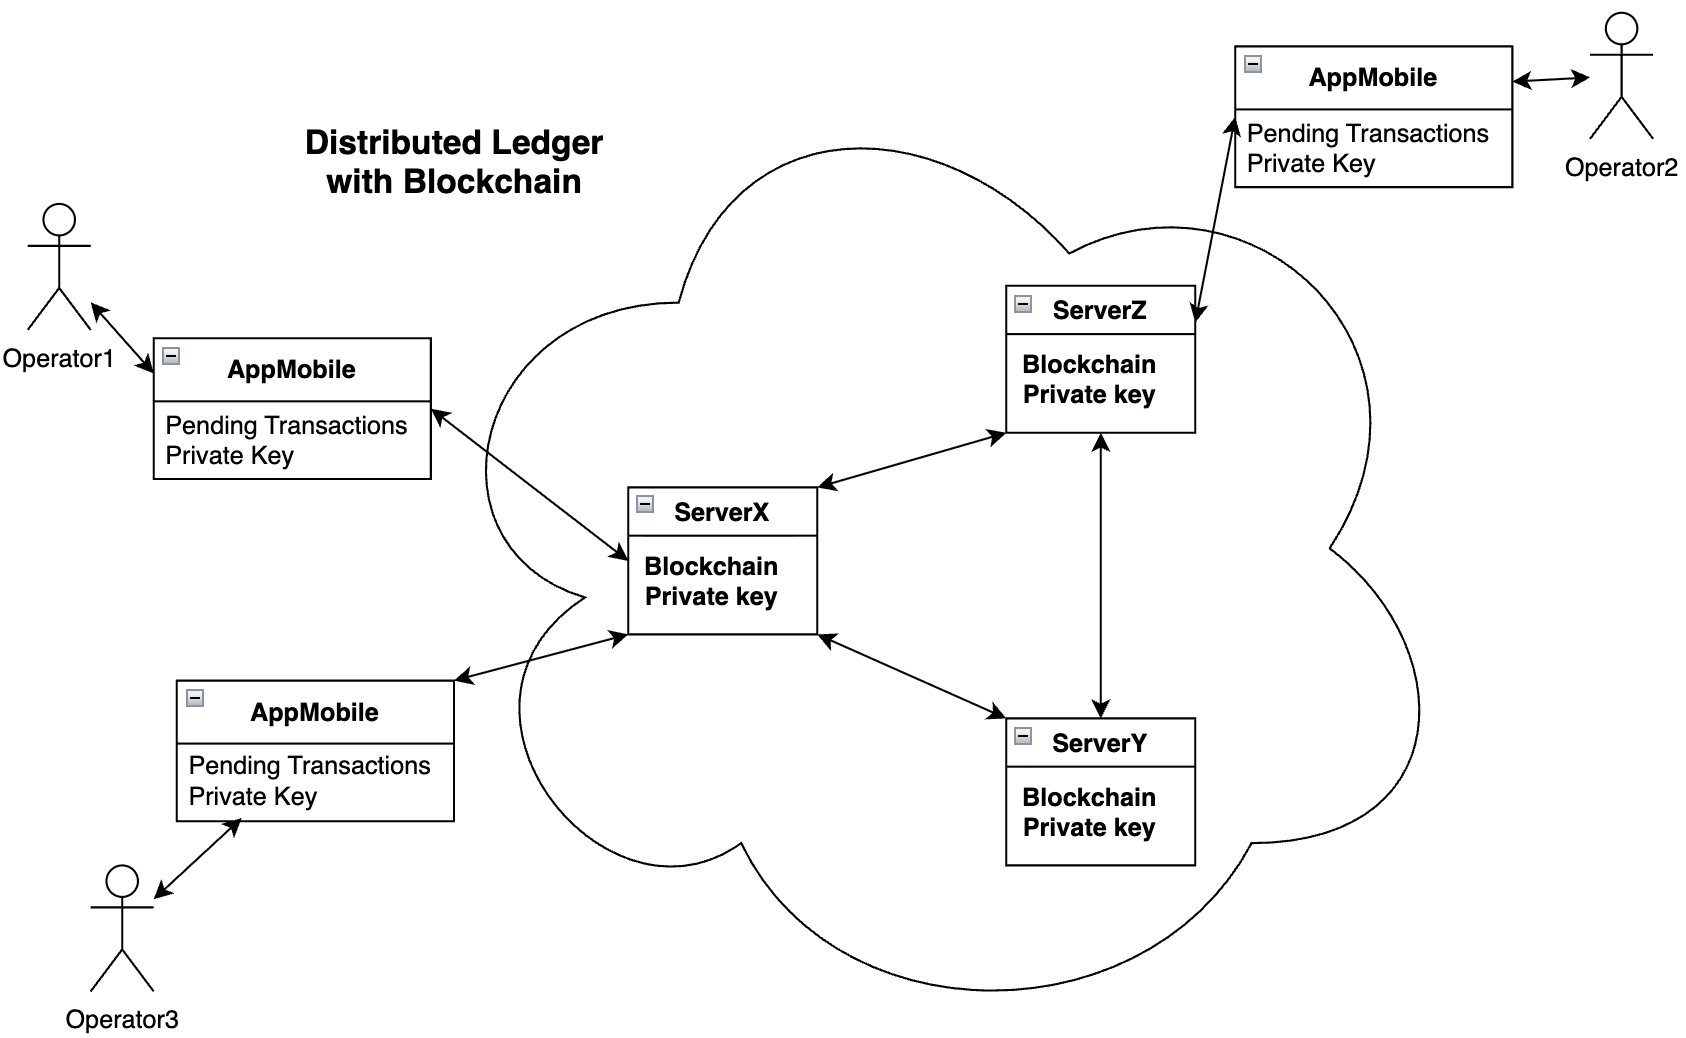
\includegraphics[width=0.75\textwidth]{UML_architettura.png}
    \caption{Logical Architecture and Component Interactions of the Distributed Ledger System.}
    \label{fig:uml_architecture}
\end{figure}

\begin{enumerate}
    \item \textbf{Presentation / Client Layer:} Consists of client software executed in business or personal devices operated by warehouse workers ($\text{Operator}_1, \text{Operator}_2, \dots$). It manages local key pairs, captures user input, constructs transaction structures, signs payloads, and submits them to accessible validator nodes.
    \item \textbf{Blockchain / Backend Layer:} The decentralized core comprising interconnected validator servers ($\text{Server}_X, \text{Server}_Y, \text{Server}_Z$). Each server houses:
    \begin{itemize}
        \item \emph{Mempool Manager:} Holds pending, unconfirmed transactions.
        \item \emph{Consensus Engine:} Executes the Proof of Authority / BFT protocol.
        \item \emph{State Machine Replication (SMR) Module:} Applies verified blocks to update local inventory state tables.
        \item \emph{Ledger Storage:} Append-only disk storage containing linked blocks and indexed databases for fast state queries.
    \end{itemize}
\end{enumerate}

\section{Protocols and Algorithms}

\subsection{Transaction Lifecycle and Block Proposal}
The step-by-step operational flow for inventory updates is illustrated in Figure~\ref{fig:uml_sequence}:

\begin{figure}[htbp]
    \centering
    \begin{subfigure}[b]{0.48\textwidth}
        \centering
        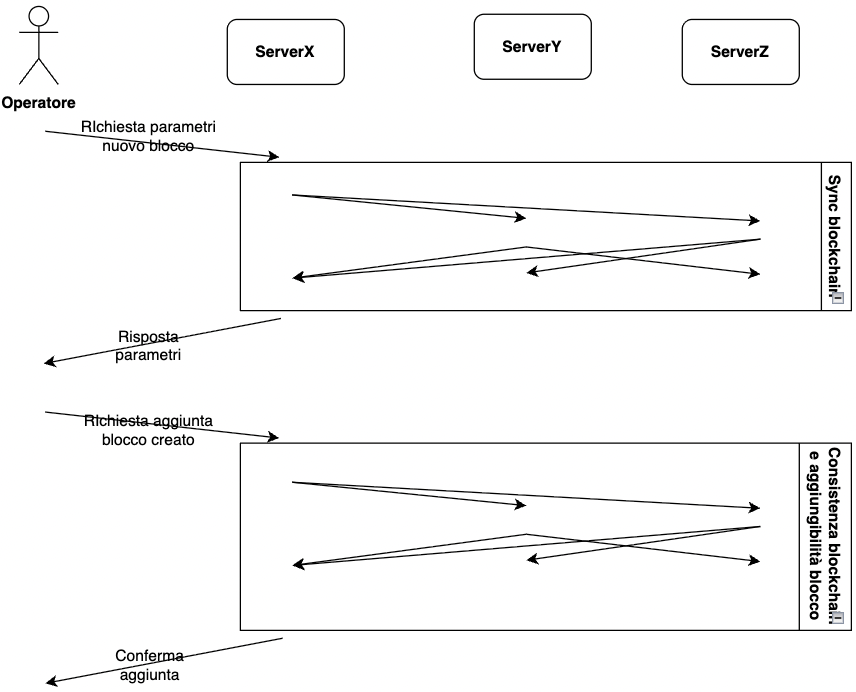
\includegraphics[width=\textwidth]{UML_attivita.png}
        \caption{Sequence Diagram: Transaction Submission \& Validation.}
        \label{fig:uml_seq1}
    \end{subfigure}
    \hfill
    \begin{subfigure}[b]{0.48\textwidth}
        \centering
        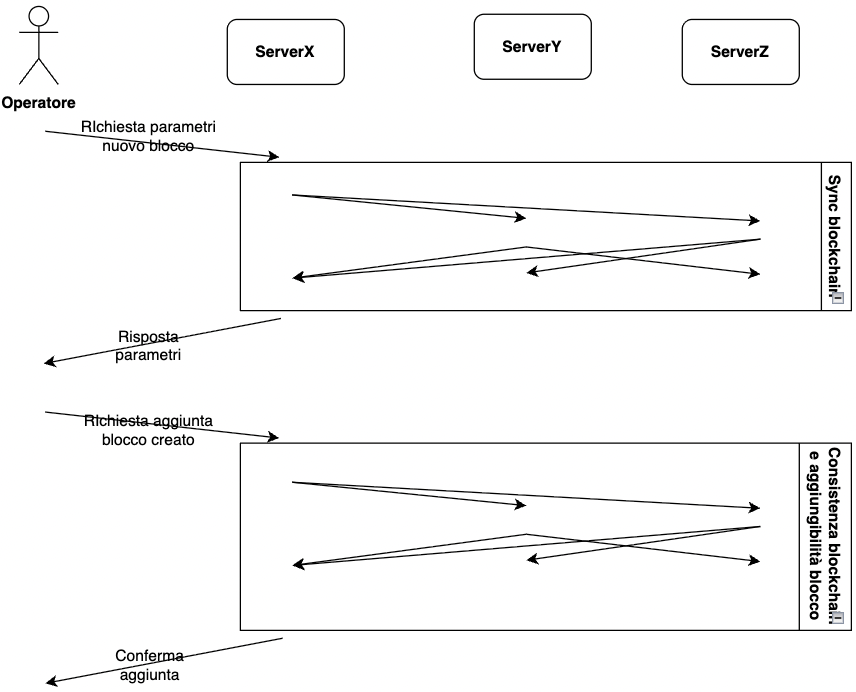
\includegraphics[width=\textwidth]{UML_attivita.png}
        \caption{Sequence Diagram: Consensus Block Propagation.}
        \label{fig:uml_seq2}
    \end{subfigure}
    \caption{UML Sequence Diagrams outlining component interactions during operation execution.}
    \label{fig:uml_sequence}
\end{figure}

\begin{enumerate}
    \item \textbf{Submission:} Client node drafts transaction $T = \langle \text{Type}, \text{AssetID}, \text{Qty}, \text{Timestamp}, \text{Sig}_{\text{Op}} \rangle$ and sends it to $\text{Server}_X$.
    \item \textbf{Broadcast \& Pooling:} $\text{Server}_X$ validates $\text{Sig}_{\text{Op}}$, checks local inventory constraints, and broadcasts $T$ to peer nodes ($\text{Server}_Y, \text{Server}_Z$).
    \item \textbf{Block Assembly:} The round leader collects pending transactions from its mempool into block candidate $B_k = \langle k, \text{Hash}(B_{k-1}), \{T_1, \dots, T_m\}, \text{Sig}_{\text{Leader}} \rangle$.
    \item \textbf{Consensus Vote:} The leader broadcasts $B_k$. Peers verify signatures, hash chain continuity, and contained transactions. If valid, peers return a pre-commit vote.
    \item \textbf{Commit \& State Update:} Upon gathering a supermajority of valid votes ($> 2/3$), nodes commit $B_k$ to disk, update the local inventory state, and send a confirmation receipt back to the client. Pending transactions are resent to the round leader in case the message is lost.
\end{enumerate}

\subsection{Error Remediation Protocol}
When an operational mistake occurs (e.g., logging 100 items inbound instead of 10), the operator initiates a compensating flow:
1. The operator press the 'correction' button inside the frontend dashboard and then selects the transaction $T_{\text{remedy}}$ to be corrected. 
2. The 
3. Supervisors sign $T_{\text{remedy}}$. Once committed via consensus, state updates correctly without erasing $T_{\text{err}}$, maintaining historical auditability.

\section{Physical Architecture and Deployment}
The physical deployment model relies on containerized microservices (Docker) across distributed sites:
\begin{itemize}
    \item Each regional warehouse hosts a local validator container connected to regional hardware security modules (HSM) for key management.
    \item Client devices connect via secure REST/gRPC endpoints exposed by local API gateways.
    \item Peer-to-peer (P2P) communication among validator containers uses encrypted TCP channels over enterprise VPN tunnels.
\end{itemize}
 while the operator screatcreates a 
\section{Development Plan}
To manage implementation risk, development is divided into three incremental tiers:

\begin{description}
    \item[\textbf{Tier 1: Minimal Viable Product (MVP)}]\hfill
    \begin{itemize}
        \item In-memory append-only blockchain storage module.
        \item Single-node API server with basic CLI client for inbound/outbound logging.
        \item Cryptographic signature generation and SHA-256 block linking.
    \end{itemize}

    \item[\textbf{Tier 2: Distributed Consensus \& Persistence}]\hfill
    \begin{itemize}
        \item Multi-node network execution with PoA consensus implementation.
        \item Disk persistence engine (LevelDB/RocksDB) for state recovery.
        \item Compensating transaction protocol for error remediation.
    \end{itemize}

    \item[\textbf{Tier 3: Advanced Features \& Fault Injection}]\hfill
    \begin{itemize}
        \item Web-based dashboard interface for warehouse operators.
        \item Role-Based Access Control (RBAC) certificate verification module.
        \item Simulated Byzantine fault injection framework for robustness testing under network partition and node crash conditions.
    \end{itemize}
\end{description}

% ==============================================================================
% REMAINING CHAPTER STUBS (FOR FUTURE IMPLEMENTATION)
% ==============================================================================
\chapter{Implementation}\label{ch:implementation}
\textit{[Implementation details regarding platform selection, specific data structures, middleware bindings, and codebase organization will be detailed here in future revisions.]}

\chapter{Validation}\label{ch:validation}
\textit{[Performance benchmarks, TPS throughput graphs, fault tolerance simulation results, and UI screenshots validating the requirements of Chapter~\ref{ch:analysis} will be presented here.]}

\chapter{Conclusions}\label{ch:conclusions}
\textit{[Summary of achieved milestones, comparison against original objectives, and proposed future work.]}

\appendix
\chapter{Source Code and Setup Instructions}\label{ch:appendix}
\textit{[Build instructions, environment configuration scripts, snapshot images and key code snippets.]}

\end{document}